\documentclass{article} % For LaTeX2e
\usepackage{nips14submit_e,times}
\usepackage{amsmath}
\usepackage{amsthm}
\usepackage{amssymb}
\usepackage{mathtools}
\usepackage{hyperref}
\usepackage{url}
\usepackage{algorithm}
\usepackage[noend]{algpseudocode}
%\documentstyle[nips14submit_09,times,art10]{article} % For LaTeX 2.09

\usepackage{mathrsfs}
\usepackage{graphicx}
\usepackage{caption}
\usepackage{subcaption}

\def\eQb#1\eQe{\begin{eqnarray*}#1\end{eqnarray*}}
\def\aB#1\aE{\begin{align*}#1\end{align*}}
\def\eQnb#1\eQne{\begin{align}#1\end{align}}
\providecommand{\e}[1]{\ensuremath{\times 10^{#1}}}
\providecommand{\pb}[0]{\pagebreak}

\newcommand{\E}{\mathrm{E}}
\newcommand{\Var}{\mathrm{Var}}
\newcommand{\Cov}{\mathrm{Cov}}

\def\Qb#1\Qe{\begin{question}#1\end{question}}
\def\Sb#1\Se{\begin{solution}#1\end{solution}}

\newenvironment{claim}[1]{\par\noindent\underline{Claim:}\space#1}{}
\newtheoremstyle{quest}{\topsep}{\topsep}{}{}{\bfseries}{}{ }{\thmname{#1}\thmnote{ #3}.}
\theoremstyle{quest}
\newtheorem*{definition}{Definition}
\newtheorem*{theorem}{Theorem}
\newtheorem*{lemma}{Lemma}
\newtheorem*{question}{Question}
\newtheorem*{preposition}{Preposition}
\newtheorem*{exercise}{Exercise}
\newtheorem*{challengeproblem}{Challenge Problem}
\newtheorem*{solution}{Solution}
\newtheorem*{remark}{Remark}
\usepackage{verbatimbox}
\usepackage{listings}
\title{Harmonic Analysis:  \\
Problem Set II}


\author{
Youngduck Choi \\
CIMS \\
New York University\\
\texttt{yc1104@nyu.edu} \\
}


% The \author macro works with any number of authors. There are two commands
% used to separate the names and addresses of multiple authors: \And and \AND.
%
% Using \And between authors leaves it to \LaTeX{} to determine where to break
% the lines. Using \AND forces a linebreak at that point. So, if \LaTeX{}
% puts 3 of 4 authors names on the first line, and the last on the second
% line, try using \AND instead of \And before the third author name.

\newcommand{\fix}{\marginpar{FIX}}
\newcommand{\new}{\marginpar{NEW}}

\nipsfinalcopy % Uncomment for camera-ready version

\begin{document}


\maketitle

\begin{abstract}
This work contains solutions to the problem set III
of Harmonic Analysis 2016 at Courant Institute of Mathematical Sciences.
\end{abstract}

\begin{question}[1]
\hfill
\begin{figure}[h!]
  \centering
    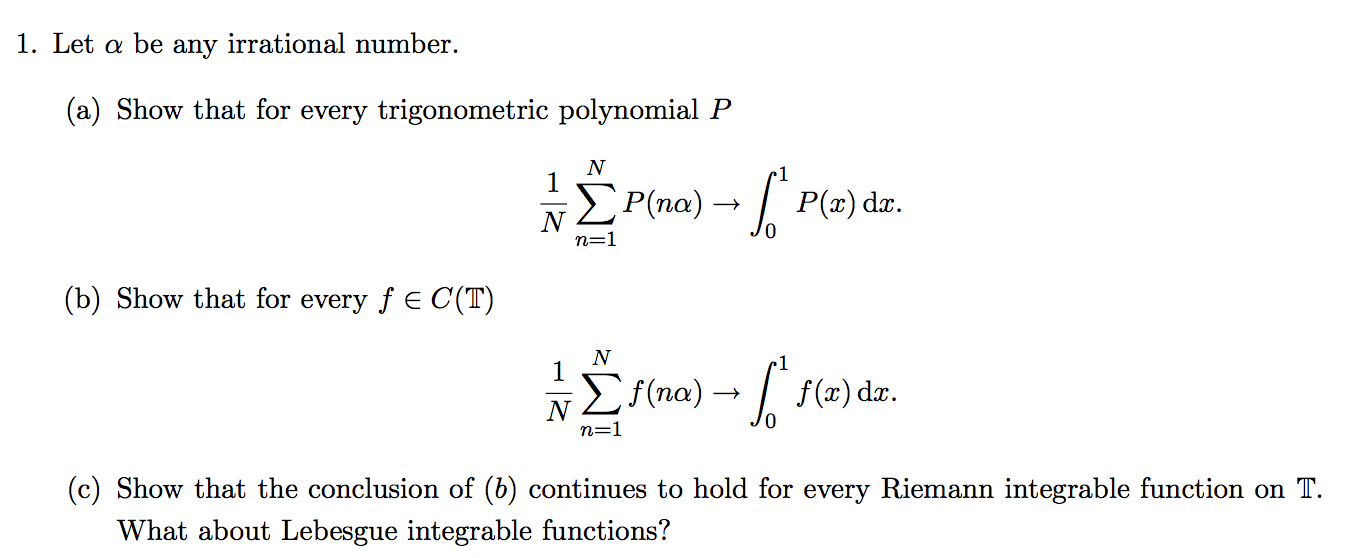
\includegraphics[width=0.8\textwidth]{HA-3-1.png}
\end{figure}
\end{question}
\begin{solution} \hfill \\
Throughout this problem, a domain of any function will be consistently defined as $\mathbb{T}$. \\
\textbf{(a)}
Let $\alpha$ be a irrational number. First, consider $e(k x)$. For $k = 0$, we have $1$ converges to $1$.
Now, for any $k \neq 0$, we have that $\int_{0}^{1} e(k x) = 0$. Furthermore, as $\alpha$ is 
an irrational, we have that $e(k \alpha ) \neq 1$. Hence, by the geometric series formula,
it follows that
\eQb
\dfrac{1}{N} \sum_{n=1}^{N} e(n\alpha ) &=& \dfrac{e(k\alpha)}{N}
\dfrac{1-e(k N \alpha )}{1-e(k\alpha)}, 
\eQe
which converges to $0$ as $N \to \infty$. Therefore, we have shown the convergence holds true
for exponentials. As trig polynomials are finite linear combinations of exponentials, 
by the linearity of limit, the convergence is true for any trig polynomial.

\bigskip

\textbf{(b)}
Fix $\epsilon > 0$. 
It follows that
By the density of trig polynomials in $C(\mathbb{T})$, there exists a polynomial $P$ such that
$||P - f||_{max} < \epsilon$. By part $(a)$, the triangle inequality, and rules of
integration, it follows that, 
\eQb
\left| \dfrac{1}{N} \sum_{n=1}^{N} f(n \alpha) - \int_{0}^{1} f(x) dx \right| 
&\leq&   
\left| \dfrac{1}{N} \sum_{n=1}^{N} f(n \alpha) 
- \dfrac{1}{N} \sum_{n=1}^{N} P(n \alpha) \right| \\
&+&  
\left| \dfrac{1}{N} \sum_{n=1}^{N} P(n \alpha)  
- \int_{0}^{1} P(x) dx \right| \\
&+& \left| \int_{0}^{1} P(x) dx  
- \int_{0}^{1} f(x) dx \right| \\ 
&\leq&   
\dfrac{1}{N} \sum_{n=1}^{N} |f(n \alpha) 
-P(n \alpha)| \\
&+&  
\left| \dfrac{1}{N} \sum_{n=1}^{N} P(n \alpha)  
- \int_{0}^{1} P(x) dx \right| \\
&+&  \int_{0}^{1} |P(x) - f(x)| dx < \epsilon + \epsilon + \epsilon = 3\epsilon, 
\eQe
for all $N$ large enough. Hence, we have shown that the convergence holds true for
all continuous functions.

\bigskip

\textbf{(c)} Before proceeding to the main part of the proof, we prove that the
asserted convergence holds true for all characteristic functions of $(a,b) \in \mathbb{T}$,
which is quite natural as the definition of Riemann integration involves a partition with
the associated upper sum and lower sum:
\begin{equation}\label{eq:convergence1}
\dfrac{1}{N} \sum_{n=1}^{N} \chi_{(a,b)}(n\alpha) \to \int_{0}^{1} 
\chi_{(a,b)}(x) dx , \> \text{ as } \> N \to \infty.
\end{equation}
Fix $\epsilon > 0$, and $(a,b) \in \mathbb{T}$. Let $f_{\epsilon}^{+}$ and $f_{\epsilon}^{-}$
be continuous functions on $\mathbb{T}$, defined by
\eQb
f_{\epsilon}^{+}(x) &=& 
\left\{
    \begin{array}{ll}
        0  & \mbox{if } x \in [0,a - \epsilon) \\
        \frac{1}{\epsilon}(x-a) + 1 & \mbox{if } x \in [a-\epsilon, a) \\   
        1 & \mbox{if } x \in [a,b) \\ 
        -\frac{1}{\epsilon}(x-b) + 1 & \mbox{if } x \in [b, b+\epsilon) \\   
        0 & \mbox{if } x \in [b + \epsilon,1], \\
    \end{array}
\right.
\eQe
and
\eQb
f_{\epsilon}^{-}(x) &=& 
\left\{
    \begin{array}{ll}
        0  & \mbox{if } x \in [0,a) \\
        \frac{1}{\epsilon}(x-a)  & \mbox{if } x \in [a , a + \epsilon) \\   
        1 & \mbox{if } x \in [a+\epsilon,b-\epsilon) \\ 
        -\frac{1}{\epsilon}(x-b)  & \mbox{if } x \in [b-\epsilon, b) \\   
        0 & \mbox{if } x \in [b,1]. \\
    \end{array}
\right.
\eQe
In particular, we have
\begin{equation} \label{eq:bound1}
b - a - 2\epsilon \leq \int_{0}^{1} f_{\epsilon}^{-}(x) dx \> \text{ and } \>
\int_{0}^{1} f_{\epsilon}^{+}(x) dx \leq b - a + 2\epsilon,
\end{equation}
along with
\begin{equation} \label{eq:bound2} 
\dfrac{1}{N} \sum_{n=1}^{N} f_{\epsilon}^{-}(n\alpha) \leq 
\dfrac{1}{N} \sum_{n=1}^{N} \chi_{(a,b)}(n\alpha) \leq
\dfrac{1}{N} \sum_{n=1}^{N} f_{\epsilon}^{+}(n\alpha). 
\end{equation} 
Now, letting $N \to \infty$ on 
both sides of $\eqref{eq:bound2}$ respectively, we obtain
\eQb
b - a - 2\epsilon \leq \liminf_{N \to \infty} 
\dfrac{1}{N} \sum_{n=1}^{N} \chi_{(a,b)}(n\alpha) 
 \> \text{ and } 
\> \limsup_{N \to \infty}  
\dfrac{1}{N} \sum_{n=1}^{N} \chi_{(a,b)}(n\alpha)
\leq b -a + 2\epsilon. 
\eQe
As $\epsilon$ was arbitrary, we have shown that the asserted convergence is true for
all characteristic functions in $\mathbb{T}$. As before, the result can be extended
to all finite linear combinations of characteristic functions. 

\smallskip

We proceed to the main part of the proof. Fix $\epsilon > 0$. 
As $f$ is Riemann integrable, taking a fine enough partition, we have 
\eQb
\int_{0}^{1} f(x) dx - \epsilon \leq \int_{0}^{1} L_f(dx) \> \text{ and } 
\> 
\int_{0}^{1} U_f(x) dx \leq \int_{0}^{1} f(x) dx + \epsilon, 
\eQe
with 
\eQb
\dfrac{1}{N} \sum_{i=1}^{N} L_{f}(n\alpha) \leq \dfrac{1}{N} \sum_{i=1}^{N}
f(n\alpha) \leq \dfrac{1}{N} \sum_{i=1}^{N} U_{f}(n\alpha),
\eQe
where $U_f$, and $L_f$ denote the upper, lower Riemann sum of the chosen partition
respectively. In view of \eqref{eq:convergence1}, letting $N \to \infty$,  
we obtain
\eQb
\int_{0}^{1} f(x) dx - \epsilon 
\leq \liminf_{N \to \infty} 
\dfrac{1}{N} \sum_{i=1}^{N} f(n\alpha) \> \text{ and } \> 
\limsup_{N \to \infty} 
\dfrac{1}{N} \sum_{i=1}^{N} f(n\alpha) \leq 
\int_{0}^{1} f(x) dx + \epsilon.
\eQe 
As $\epsilon$ was arbitrary, we have shown that the asserted convergence is true for
all Riemann integrable functions on $\mathbb{T}$.

\smallskip

Now, for the case of Lebesgue integration, consider $\chi_{A}$, where
$A = \{ <n \alpha> \> | \> n \in \mathbb{N}\}$.  

\end{solution}

\newpage

\begin{question}[2]
\hfill
\begin{figure}[h!]
  \centering
    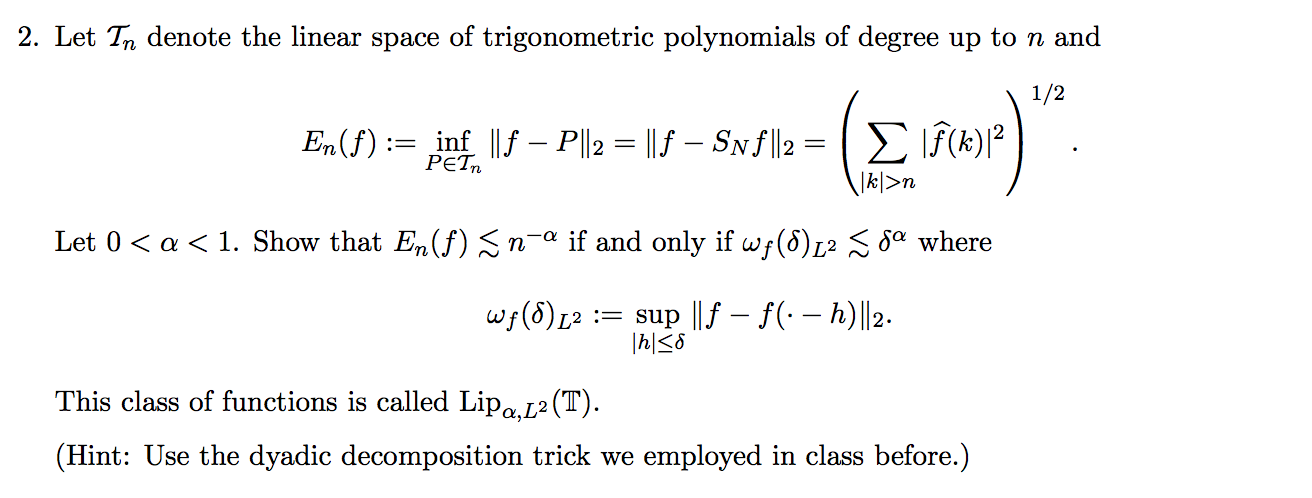
\includegraphics[width=1\textwidth]{HA-3-2.png}
\end{figure}
\end{question}
\begin{solution}
\end{solution}

\bigskip

\begin{question}[3]
\hfill
\begin{figure}[h!]
  \centering
    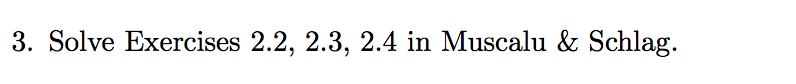
\includegraphics[width=0.5\textwidth]{HA-3-3.png}
\end{figure}
\end{question}
\begin{solution} 
\hfill $\qed$
\end{solution}

\bigskip

\begin{question}[4]
\hfill
\begin{figure}[h!]
  \centering
    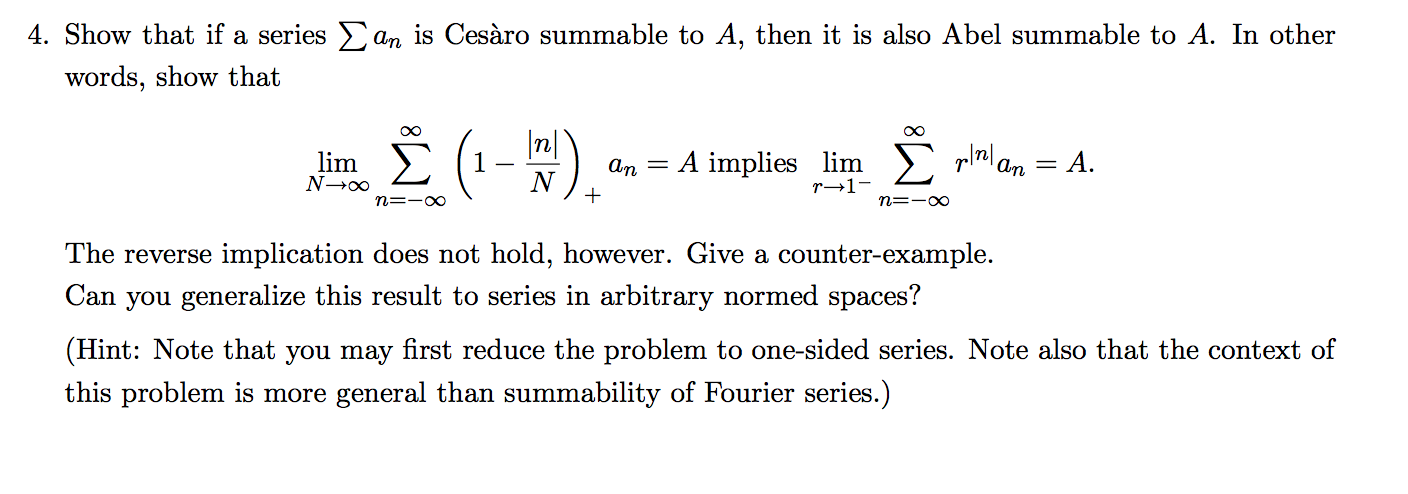
\includegraphics[width=1\textwidth]{HA-3-4.png}
\end{figure}
\end{question}
\begin{solution} \hfill \\
 
\hfill $\qed$
\end{solution}

\bigskip


\end{document}
